\documentclass[letterpaper]{scrartcl}

\usepackage{uog}
\usepackage[framemethod=TikZ]{mdframed}

\mdfdefinestyle{MyFrame}{%
    linecolor=triton_green,
    outerlinewidth=2.5pt,
    roundcorner=15pt,
    innertopmargin=\baselineskip,
    innerbottommargin=\baselineskip,
    innerrightmargin=15pt,
    innerleftmargin=15pt,
    backgroundcolor=triton_green!25!white!10}



%\newcommand\sourceURL{https://www.overleaf.com/read/xmyythnqhymz}
\newcommand\docID{2018-Oct-001}
\newcommand\createdOn{30 August, 2018}

\begin{document}
    \title{\color{triton_green}\textbf{Minerva Statistical Consulting},\\ \textit{\textbf{Bulletin for the UK Housing Market}}}
    \author{\color{triton_green}\textbf{Jonathan Miller}}
    \date{}
\AddToShipoutPictureBG*{%
  \AtTextLowerLeft{%
    \makebox[\textwidth]{%
      \raisebox{\dimexpr\textheight-\height}%
    }%
  }%
}
	\maketitle
	\section*{\color{triton_green}Greetings}
    	\textbf{\color{triton_green}169} days! What will happen on March 29, 2019 the day the UK is scheduled to \textit{divorce} from the EU? Any quick glance at political news segments will tell us tThe Royal Institution of Chartered Surveyors (RICS)hat if we know anything about this \textbf{\color{red}hot} topic, its that we do not know what the future holds for the UK. Hence, the property market is left exposed to the elements. 
    	
    	\textbf{\color{triton_green}19} weeks! According to the \textit{The Royal Institution of Chartered Surveyors (RICS)} property deals are taking on average 19 weeks to close. We have not seen this since RICS started collecting data. This bulletin, which will be delivered \textbf{[MONTHLY/QUARTERLY???]} and will provide updated charts, analysis and comparisons of what is happening in the market now. Data is sourced from the UK Land Registry website. This data represents what the \textbf{actual} price of sale. 
    	
    	In this first issue, we use seasonally adjusted data, meaning changes in the data due to season have been removed. This helps to show that a price changes is not because it is, say, a holiday or a time of year known to affect prices. The aim of this bulletin is to provide real practical data visualisations and analysis that can assist in your real estate investments and practices.
	
		
    \section*{\color{triton_green}Snap shot of the market}
        Data obtained from the UK Land Registry does lag by a month or two. Here is the latest news on the overall housing market.
        \begin{mdframed}[style=MyFrame]
        \textbf{July 2018} the average house price in the UK is \textbf{£231,422}. By comparison of \textbf{June 2018}, property prices have risen by 1.2\%. We see a rise of 3.1\% since last year. 
        \end{mdframed}
    
    \section*{\color{triton_green}Seasonally Adjusted Average House Prices}
        Let us take a look at the \textbf{average houses prices} in the UK since \textbf{1995} up until \textbf{2017}. It is important to note that the UK Land Registry uses now an index and \textbf{we will explain what this index is how to use it in the next issue}. 
        \begin{figure}[H]
            \centering
            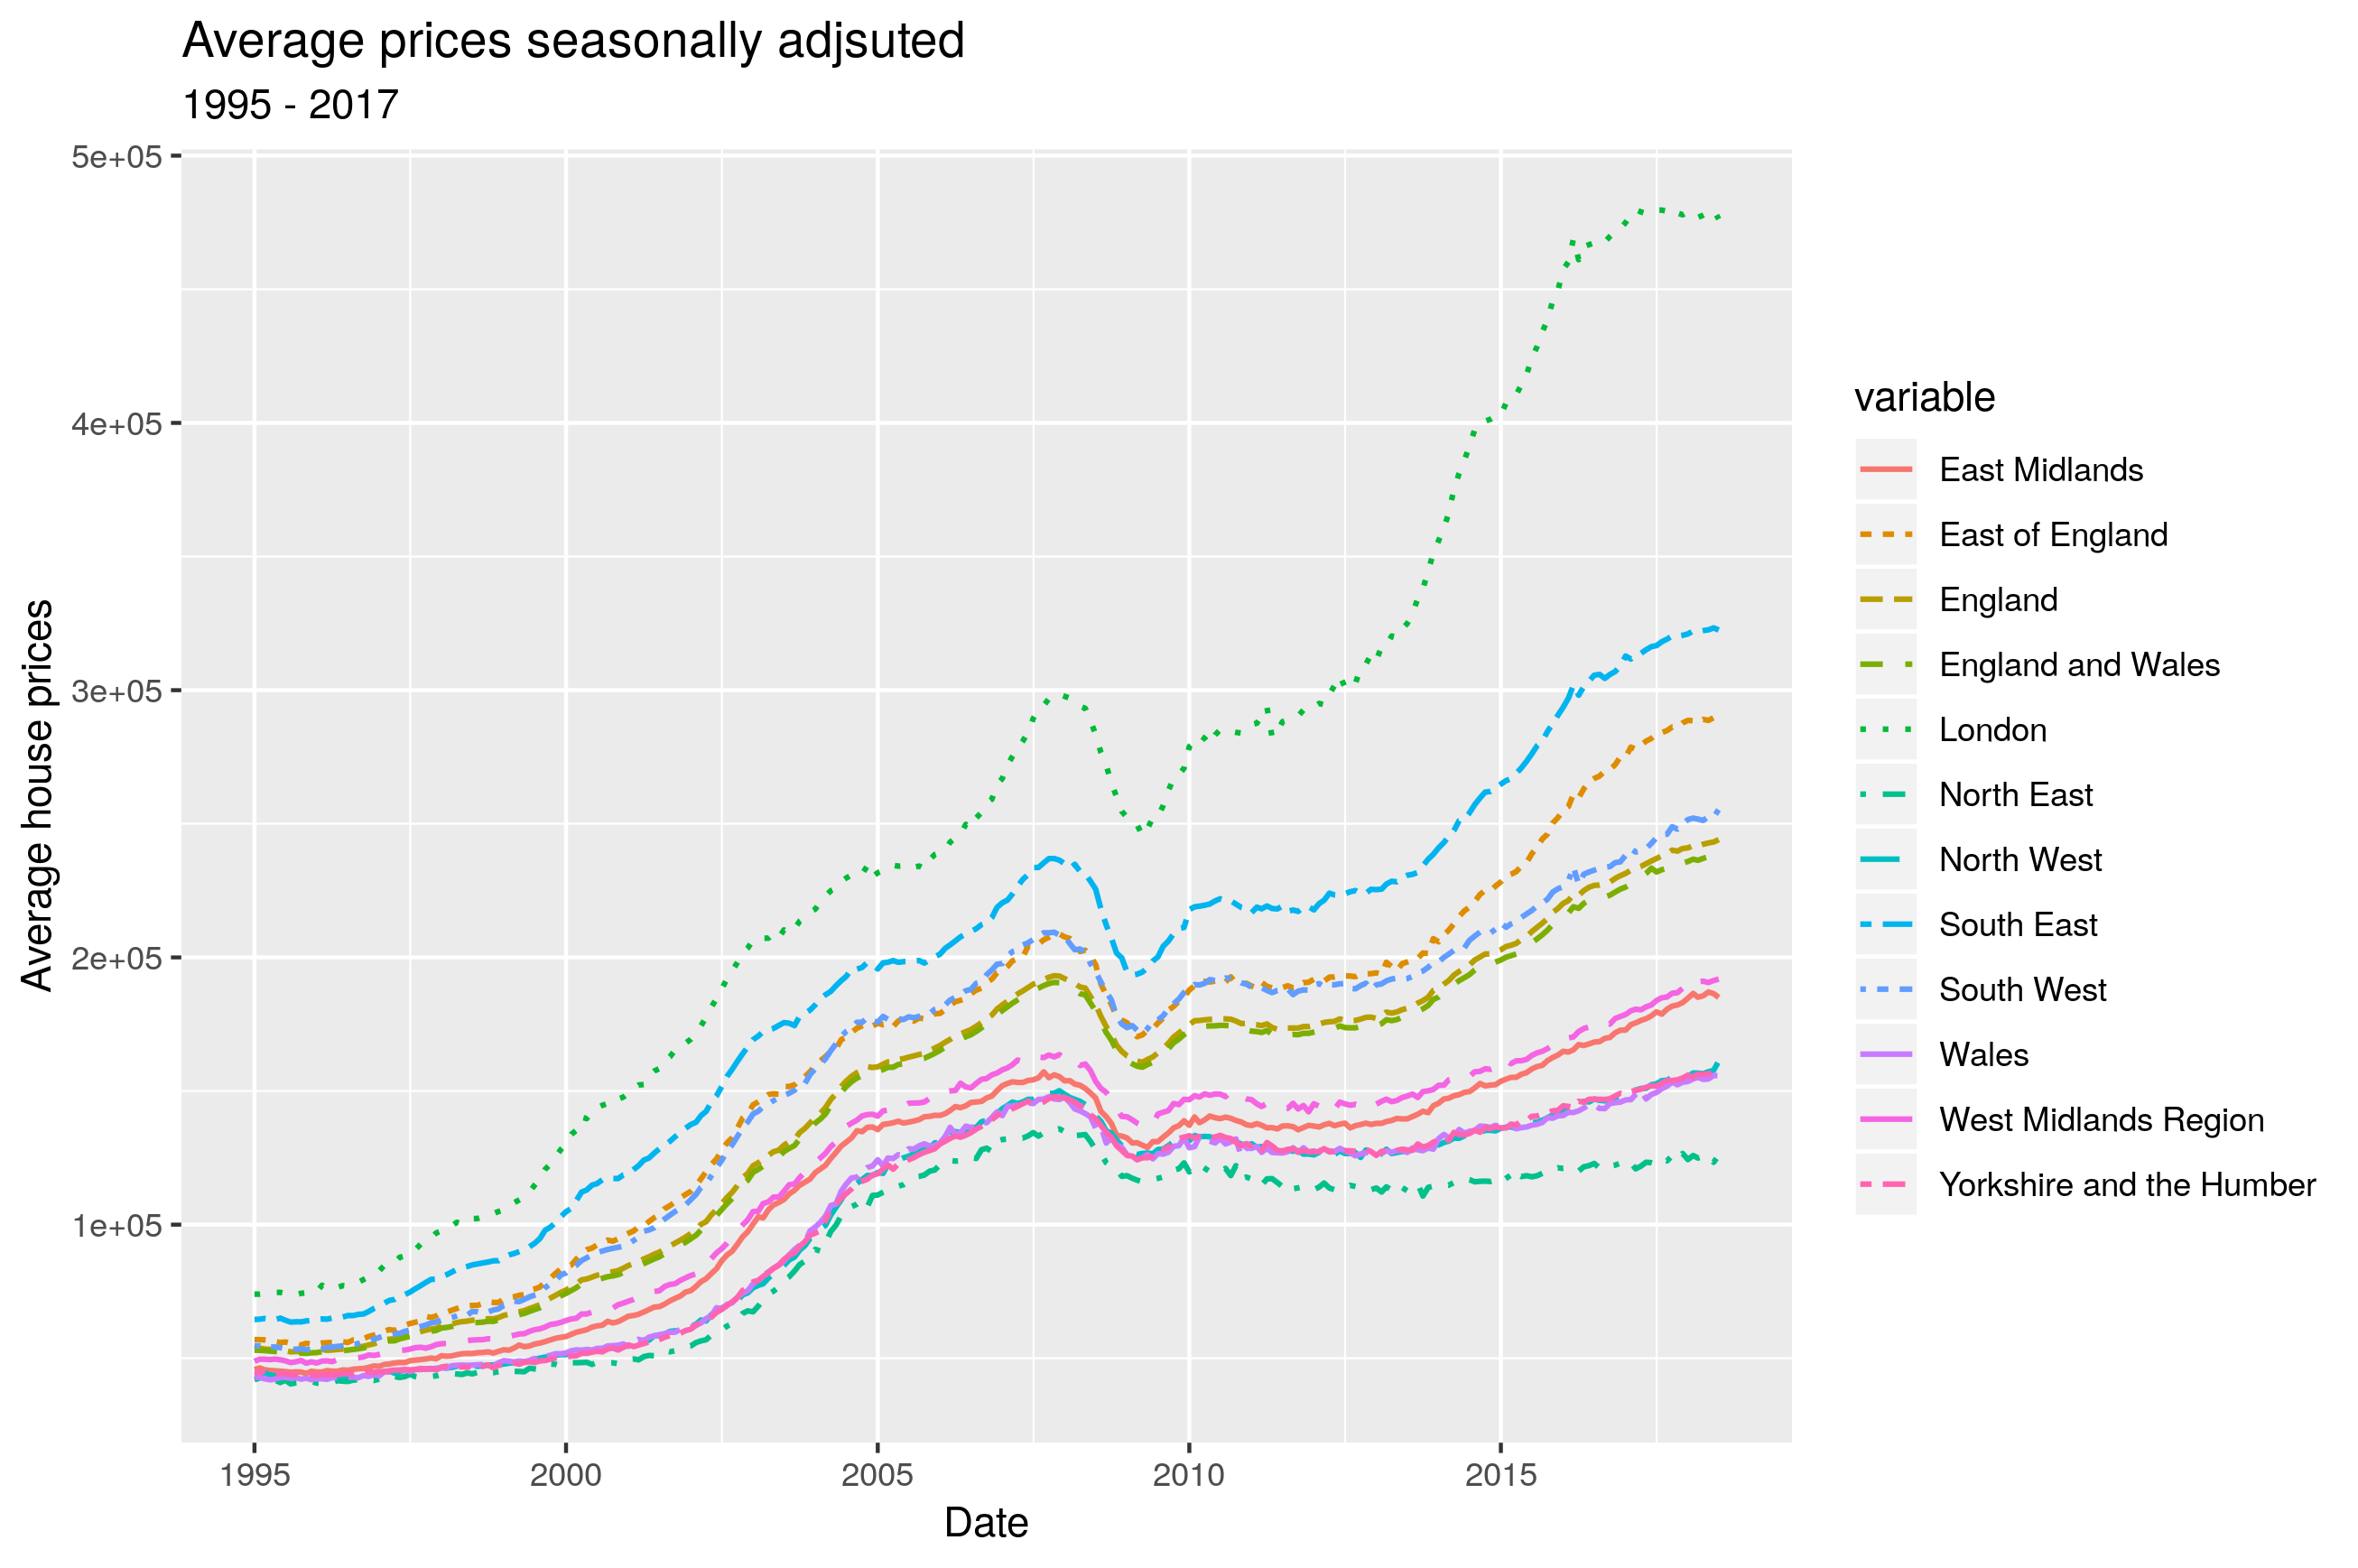
\includegraphics[width=\textwidth,keepaspectratio]{DifferentLineTypesSeriesUK.png}
            \caption{Average prices for 22 years}
            \label{fig:SA average prices}
        \end{figure}
    \subsection*{\color{triton_green}Graph analysis}
        What can be said about this image? Firstly, London out performs the rest of the UK. Secondly the country as a whole tends to move in similar paths. This indicates how connected our housing market really is. We can see the booms in housng prices as the sharper increasing slopes. For example around \textbf{2012-2015} prices all increased, whereas \textbf{2008} we see the clear representation of the Global Financial Crisis (GFC). 
        
        Further to this data, what about the trends of the data? What about cycles in the market? The trend is usually defined as the long term movement of the data. In our case, the long term movement of the housing market. Understanding the trend will help in predicting what section of the housing cycle we are currently in. A cycle is an irregulars pattern in the data in relation to the trend. 
    \subsection*{\color{triton_green}Housing price analysis as plotted over time}
    In the proceeding pages, we see data plotted with respect to the data itself, the trend and the irregular cycles found in the data.
        \begin{figure}[H]
            \centering
            \caption{The following graphs are from theses regions of the UK.}
            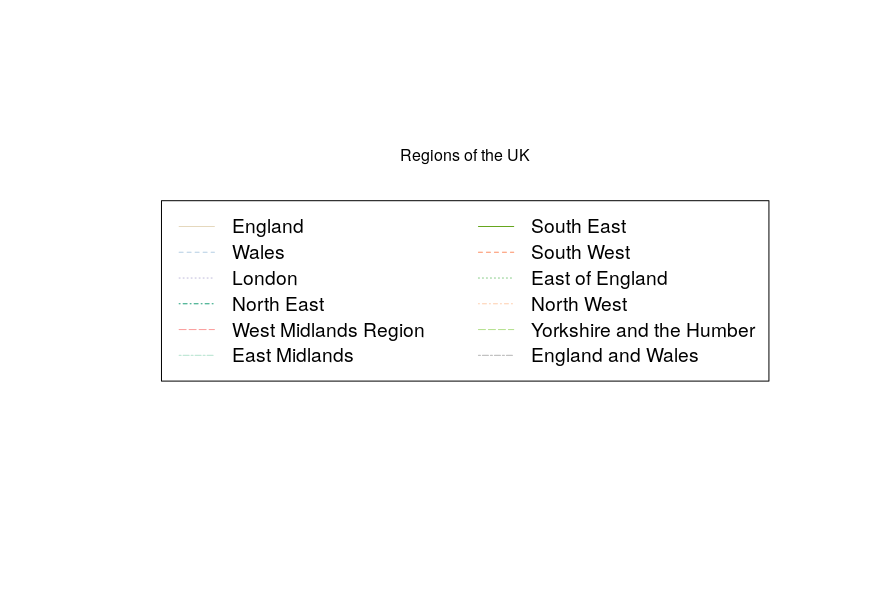
\includegraphics[scale = 0.6]{Legend.png}
            \label{fig:my_label}
        \end{figure}

        \begin{figure}[H]
            \centering
            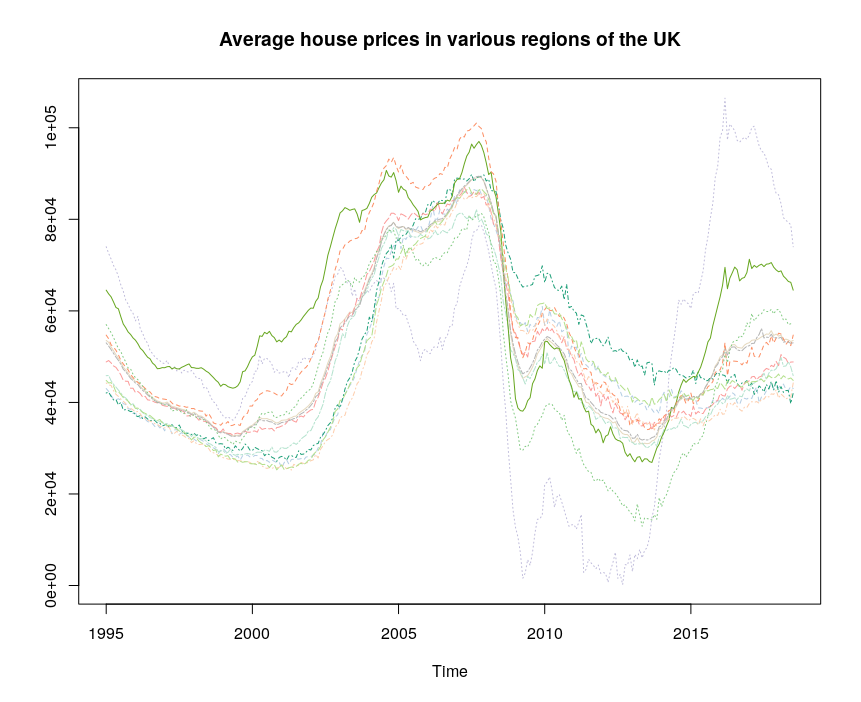
\includegraphics[scale = 0.6]{HPFilterDataNoTrendNoCycle.png}
            \caption{Average prices of homes in the UK. Notice the price decline in 2008.}
            \label{fig:my_label}
        \end{figure}
        
        \begin{figure}[H]
            \centering
            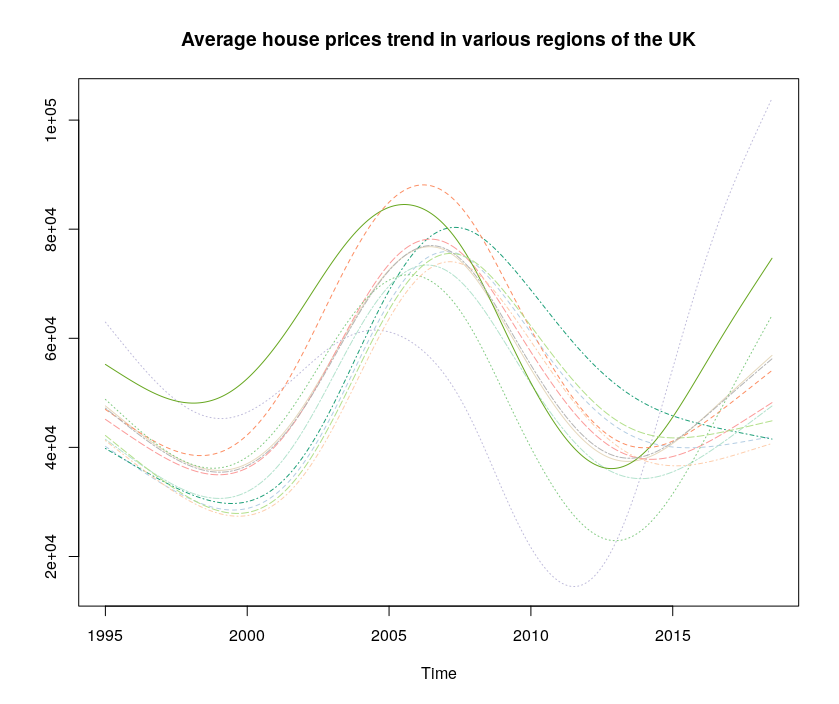
\includegraphics[scale = 0.6]{HPFilterDataTrendNoCycle.png}
            \caption{Long term trend of average prices of homes in the UK.}
            \label{fig:my_label}
        \end{figure}        
    
        \begin{figure}[H]
            \centering
            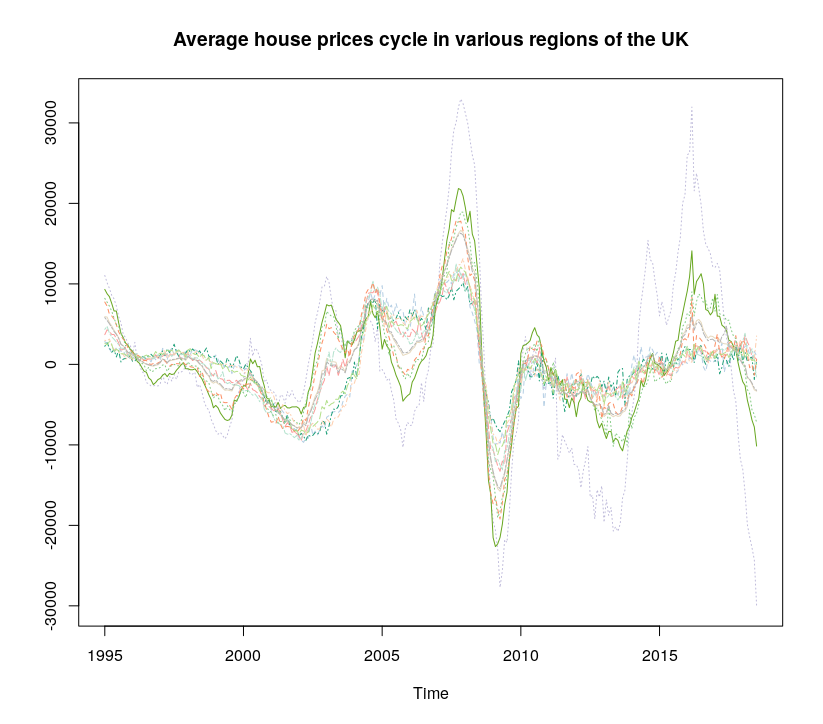
\includegraphics[scale = 0.6]{HPFilterDataNoTrendCycle.png}
            \caption{Irregular patterns of the average prices of homes in the UK.}
            \label{fig:my_label}
        \end{figure}        
    \section*{\color{triton_green}The Property Cycle}
            \begin{mdframed}[style=MyFrame]
        \textbf{The Property Cycle} 
        
        The three identifiable stages of the property cycle.
            \begin{enumerate}
                \item Boom
                \item Slump
                \item Recovery
            \end{enumerate}
            Firstly, this bulletin is not providing financial advise. Nor are we attempting to persuade the reader to make certain financial decisions. Rather, we are providing a snap shop into the data at hand. Now, there are certain observations of the property cycle. Namely, the duration with which properties are taking to complete a sale. This, along with the prices seemingly appear to be levelling out, and the media subjectivity of Brexit give ample consideration to us the writer to consider that the UK is in the slump to recovery stage of the property cycle. This is a complex situation in any time, that of determining which stage of the cycle a country or area is in, let alone with the political changes on the horizon. 
        \end{mdframed}
        \subsection*{\color{triton_green}Where to next?}
        Is it time to buy? Is it time to hold our investments? Should we consider liquidating assets? Time will only tell, and it is best to pay close attention to the data and to the media. We say to the media, in that one should aggregate what is going on and conceive an overall picture.
        \section*{\color{triton_green}Housing Price Index}
        One might notice that this data is only showing till July 2017. This is because the UK Land Registry has ceased producing data on \textit{only} seasonally adjusted data for the average prices in homes. Rather, the housing price index is the new tool to be used. This index uses what is called \textit{hehonic regression}. That just means that all of the factors that contribute to pricing a house, that can also be measured in their own right have been included into this model. The index has a numerical value. When the index was backdated to \textit{begin}, a notional valule of \textbf{0.0} was established, then based on the marked and economy in the years to follow a backdated index was formed. This gives us a current value for the index that we can use to quickly look at the health of the market. 
    \begin{mdframed}[style=MyFrame]
        \textbf{Housing Price Index (HPI)} 
        The current index is for data collected up to \textbf{August 2018}. The index is sitting at $122.1$. This is up  $0.2\%$ from last month and risen $3.2\%$ since the previous year. 
        \end{mdframed}
    \subsection*{\color{triton_green}Upcoming issues}
    In the upcoming issues, we will look at the past with respect to the HPI. We will compare this to the data in this issue and detemine best means of reading the HPI. We will also look at various methods for looking at the market and the overall health of the UK housing market.
    \section*{\color{triton_green}Subscriptions}
    For a subscription to this bulletin, please: \textbf{Here we can collaborate on some method to get subscriptions}
    
    
    % https://en.wikibooks.org/wiki/LaTeX/Bibliography_Management#Embedded_system
    %\bibliographystyle{unsrtnat}
    %\bibliography{biblio}
    
    %\begin{thebibliography}{9}

    %\bibitem{lamport94}
    %	Leslie Lamport, 1994.
    %	\textit{\LaTeX: a document preparation system},
    %	Addison Wesley, Massachusetts, 2nd edition, 1994.
        
	%\bibitem{schreiner97}
     %   Ilse H. Screiner and Donald M. Nafus, 1997.
      %  \textit{Butterflies of Micronesia},
       % University of Guam.     			\url{http://guaminsects.myspecies.info/sites/guaminsects.myspecies.info/files/ButterfliesOfMicronesia.pdf}. Accessed: 2018-02-28.

    %\end{thebibliography}
    
	%\blurb
	
\end{document}
